\section{Tumour networks} \label{s:N_I:tum}


This first validation section explores the initial hypothesis on data integration in a network approach, where edge weights are modelled proportional to the gene's mutation burden. The graph method described earlier (\cref{fig:N_I:network_pipeline}) is used to build a co-expressed graph from the gene expression of the MIBC samples, which is used to stratify TCGA cohort.

% Mention the stratification with the other methods
In addition to applying the network approach to MIBC subtyping, the results are compared to standard stratification methods: TCGA \citep{Robertson2017-mg} and the consensus \citep{Kamoun2020-tj}. Beyond comparing the derived subgroups, this comparison involves contrasting two gene selection mechanisms: the network-based approach and the selection of the most variable genes, thereby highlighting the potential of graph-based methods.

This section examines two different network sizes: 4,000 and 5,000 nodes. The first network, consisting of 4,000 genes, is used to analyse the impact of edge weight modifiers and encompasses the research on network metrics and tumour stratification in \cref{s:N_I:tum_describe,s:N_I:tum_stratification}. The second network, with 5,000 genes, is used to compare the network approach with cluster analysis in \cref{s:N_I:cs_vs_gene_sel}. A larger network is needed to compare the MIBC subtypes derived from the tumour network with those from the cluster analysis because the number of genes used to compute MEV is essential. The larger the network, the more genes are selected, leading to a larger MEV. Since the cluster analysis uses 3,500 genes, a similar number should be chosen through the network pipeline for a balanced comparison. Although more complex networks were built, they were too densely connected, which affected the performance of the Leiden algorithm (as discussed in \cref{s:N_I:sel_pruning}).

% Specifics of the network
For both networks, the genes used are selected based on relative variance (std/median) from TCGA dataset. Two modifiers, 'reward' and 'penalised,' are applied to the gene weights following the weight modifier in \cref{fig:N_I:modifiers}. Across all networks created in this section, 3 edges per gene are retained, while 6 edges per TF are maintained for TF. The top 100 genes are selected using ModCon, and the tumour dataset is employed for computing MEV scores.

% % 4K network and 5K network
% This section explores two network sizes: 4,000 and 5,000 nodes. The first network, comprising 4,000 genes, is used to study the effects of the weight modifiers on the network,\cref{s:clustering_analysis}. This network covers the work on network metrics and tumour stratification in \cref{s:N_I:tum_describe,s:N_I:tum_stratification}. A larger network of 5,000 genes is used in \cref{s:N_I:cs_vs_gene_sel}, as the Module Connective (ModCon) step selects approximately 2,800 genes, a value comparable to the 3,500 genes in the clustering analysis section.

% The decision to keep 6 edges per TF is based on findings from the experiment detailed in \cref{s:N_I:sel_pruning}. This experiment indicated that allowing more than 6 edges per TF leads to diminished returns and that all TF are included when more than 10 edges are permitted

\subsection{Network description} \label{s:N_I:tum_describe}

\begin{figure}[!t]  
\centering
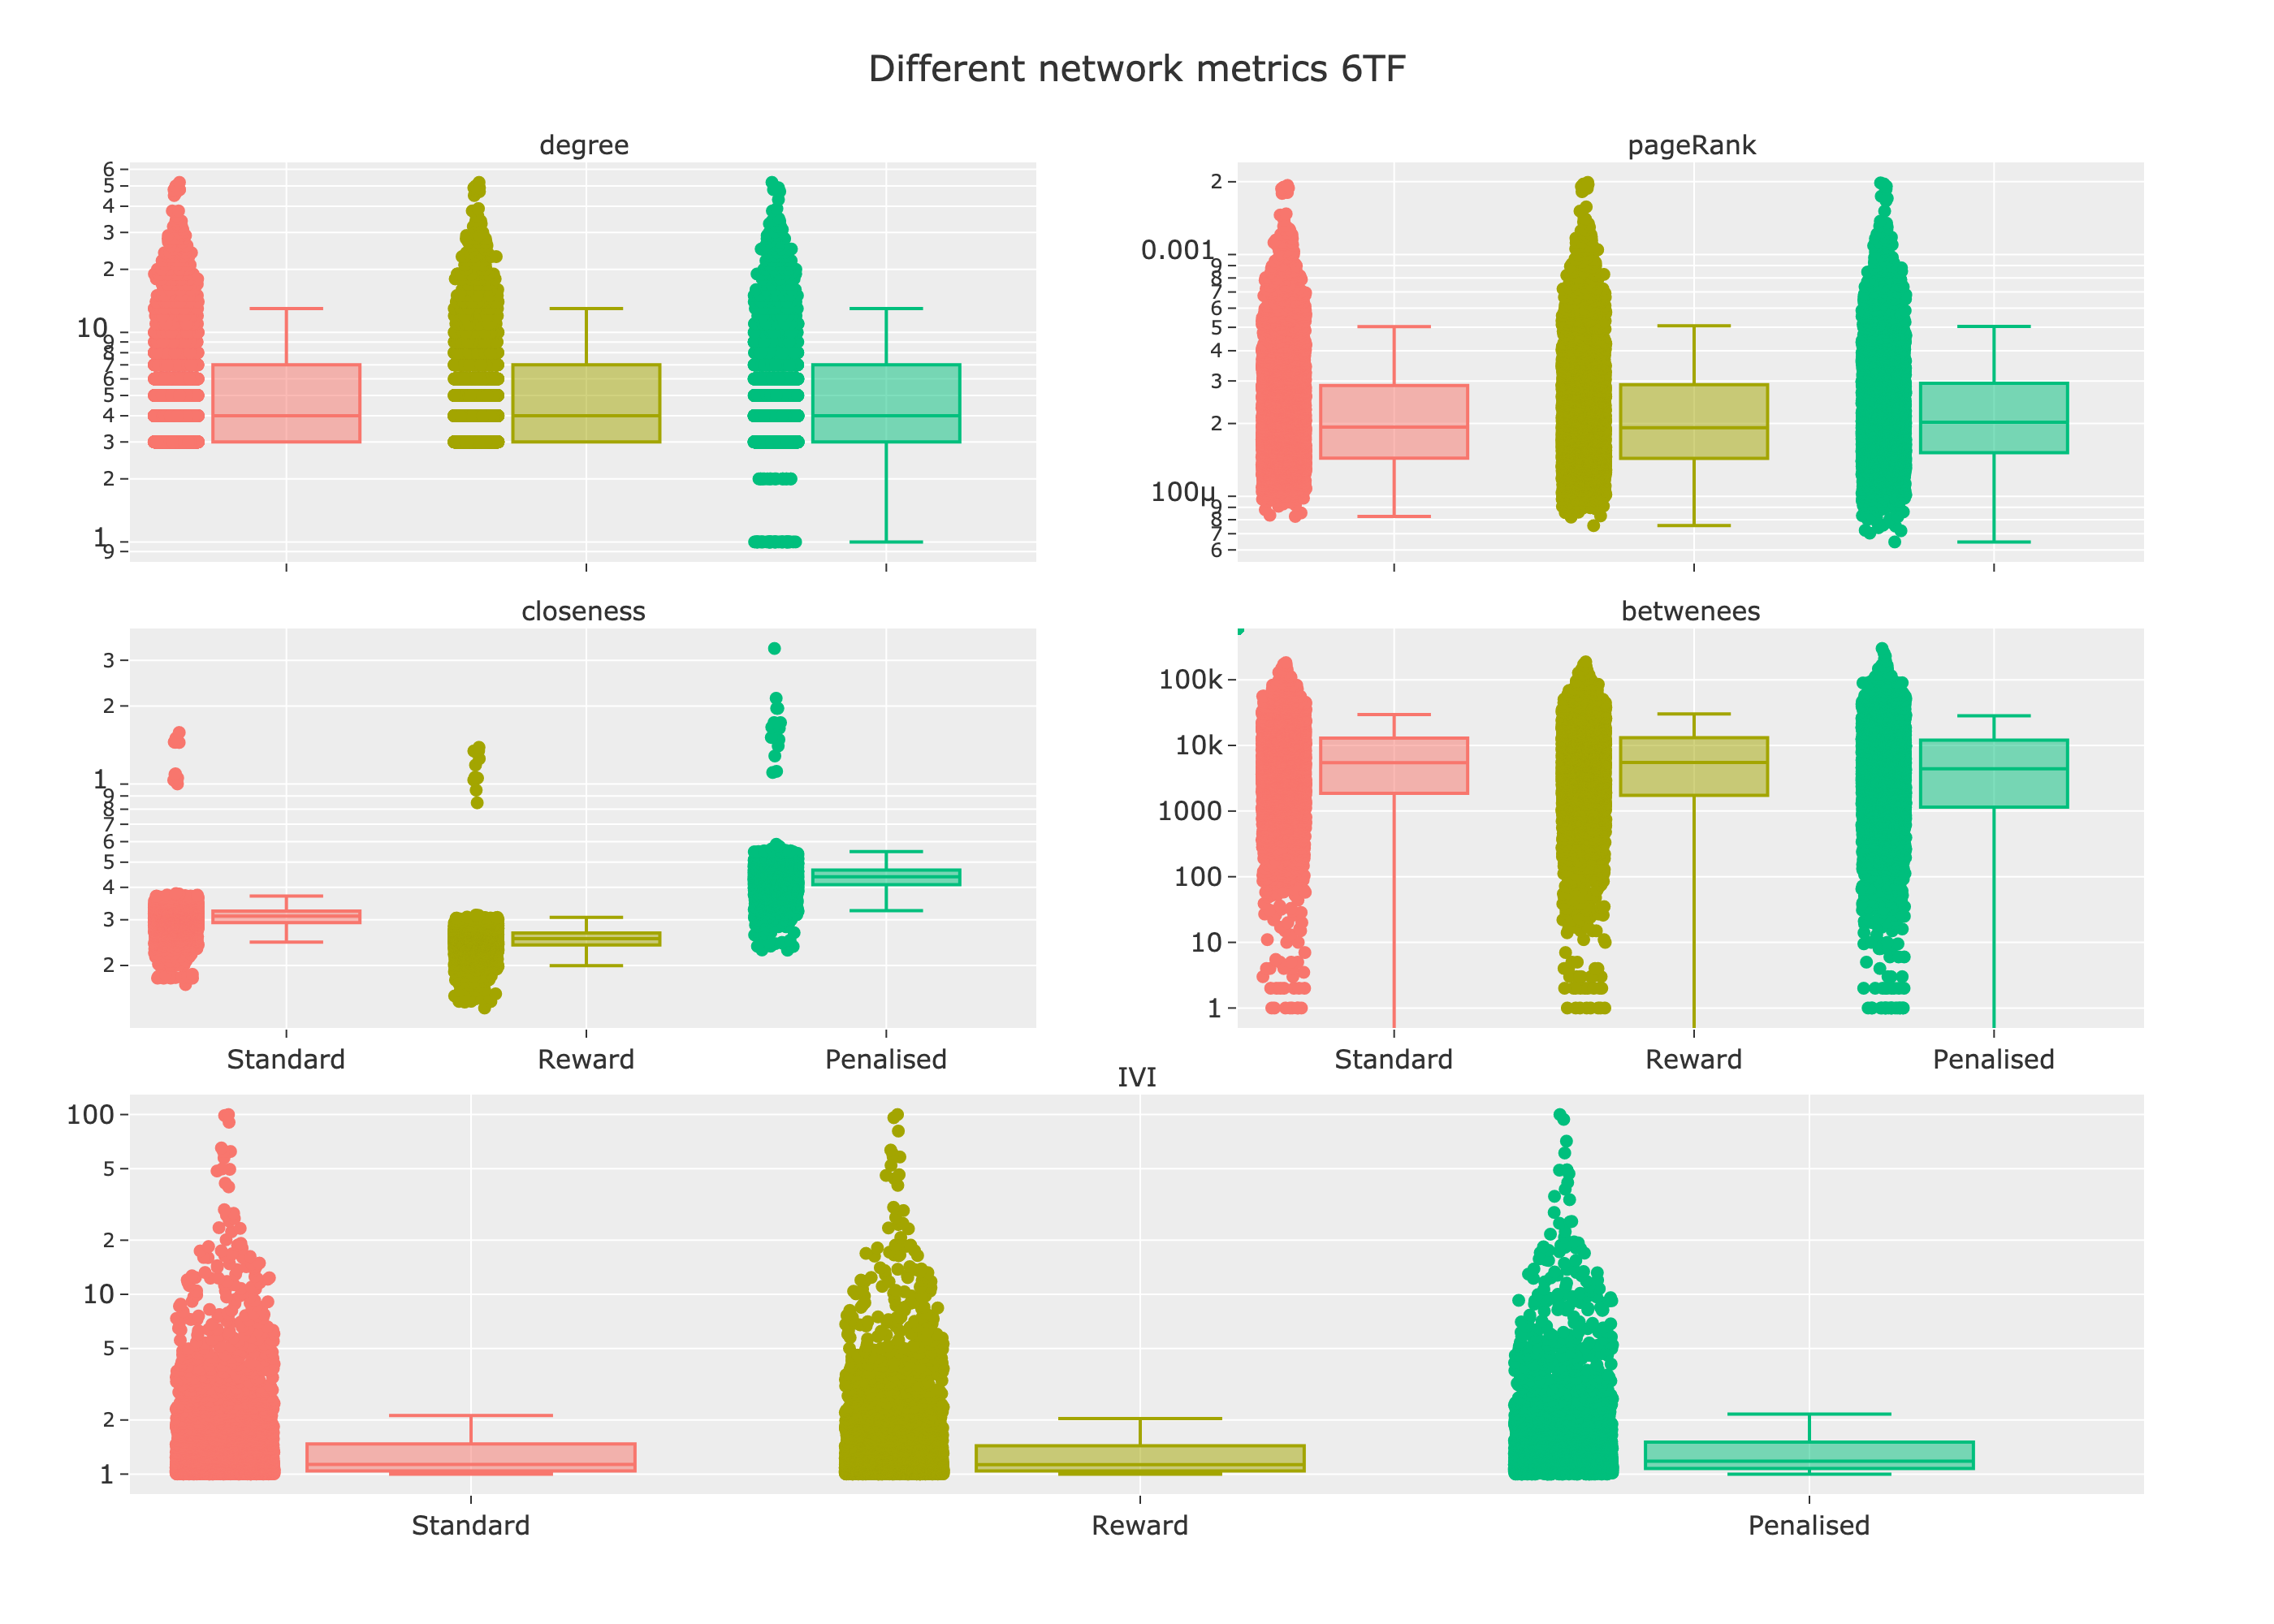
\includegraphics[width=1.0\textwidth,keepaspectratio]{Sections/Network_I/Resources/Tum_network/NetworkMetricsComp_6TF.png}
    \caption[Tum: centrality network metrics]{Distribution of node-level metrics across the three tumour networks: standard (red), reward (mustard), and penalised (green). Each network comprises 4,000 genes, with a minimum degree threshold of three connections for standard genes and six for transcription factors. The y-axis is presented on a logarithmic scale. Higher degree or PageRank values indicate greater importance of a gene/node within the network; lower closeness values suggest that nodes are more tightly connected, while higher betweenness values reflect nodes acting as key bridges between other nodes. Higher \acrlong{ivi} values indicate greater influence of a node at both local and global levels within the network. Overall, increasing edge weights (reward condition) draws nodes closer together, whereas penalising them (penalised condition) results in greater separation between nodes.
    }
    \label{fig:N_I:net_metrics_tum}
\end{figure}

% Describing the network
The graph metrics introduced in \cref{s:lit:net_metrics} are used to describe the networks built from the gene expression of TCGA samples, where scores for the standard (red), reward (mustard) and penalised (green) network are shown in \cref{fig:N_I:net_metrics_tum}. Overall, the scores exhibit the same trends across the three networks but the effects of the weight modifiers can be noticed in some of the metrics, closeness or degree.

% Difference in the penalised network
In the box plot for the degree metric, the distributions for the standard and reward are not significantly different, \acrfull{mw}: 8062709.0 with p-value: 0.53541, but how both have a lower fence and a minimum value of 3. The penalised network contains several nodes (39) with values of 1, indicating that there are isolated genes in the penalised network. This is further supported by the closeness metric across the networks, where all three graphs have a group of nodes with higher values ($>$0.7), suggesting that these nodes are further apart compared to the rest. This trend is more discernible in the penalised network, which has 17 versus 12 nodes with values more than 0.7. The isolated nodes can be explained by how the penalised modifier reduces the edge weights of the mutated genes closer to 0, as shown in \cref{fig:N_I:modifiers}.

% Reward modifiers
Rewarding the mutated genes with stronger connections has a noticeable effect on the network, see \cref{fig:N_I:net_metrics_tum}. There is significant difference (\acrshort{mw}: 15059528.0,p-value: 0.0) seen in the closeness metric, the median and lower fence values for nodes in the reward network are $0.25$ and $0.19$, respectively, compared to $0.30$ and $0.24$ in the standard network. The penalised network also affects the closeness of the nodes, having higher values and the distributions are significantly different from both the standard and reward networks; \acrfull{kw}: 9691.414,p-value: 0.0. 

% Main conclusion - effects of the reward and penalised
The two weight modifiers applied have an effect on the constructed graphs, as shown by the metrics in \cref{fig:N_I:net_metrics_tum}. From using \acrlong{mw} it appears that the penalised edge weight modifier have mostly significant changes to the standard network, while the reward non-significant, and there are significant differences between the reward and penalised networks, result shown in \cref{tab:N_I:tum_net_metrics}. Strengthening the weights brings nodes closer together, while penalising spreads the vertices further apart. 

\begin{table}[!t]
  \centering
  \small
  \begin{tabularx}{\textwidth}{>{\hsize=.25\hsize}X|>{\hsize=.35\hsize}X|>{\hsize=.35\hsize}X|>{\hsize=.35\hsize}X}
    \toprule
    \textbf{Metric} & \textbf{Standard vs Reward} & \textbf{Standard vs Penalised} & \textbf{Reward vs Penalised} \\
    \midrule
    \textbf{Betweenness} & 7998031.0;  0.985 & 8447400.0;  $9.34e^{-9}$ & 8437222.5;  $1.68e^{-8}$ \\
    \midrule
    \textbf{Closeness} & 15059528.0;  0.0 & 281163.0;  0.0 & 93297.0;  0.0 \\
    \midrule
    \textbf{Degree} & 8062709.0;  0.535 & 7864292.5;  0.982 & 7802986.0;  0.555 \\
    \midrule
    \textbf{PageRank} & 8076267.0;  0.460 & 7551878.0;  0.00235 & 7488446.0;  0.000248 \\
    \midrule
    \textbf{IVI} & 8135410.0;  0.190 & 6891664.5;  $1.77e^{-21}$ & 6747375.5;  $8.00e^{-28}$ \\
    \bottomrule
  \end{tabularx}
  \caption[Tum: Network metrics MW test]{Tumour network metrics comparison of Betweenness, Closeness, Degree, PageRank, and IVI metrics across standard, reward, and penalised networks. The first value is represented by the result from the \acrlong{mw} while the second the p-value}
  \label{tab:N_I:tum_net_metrics}
\end{table}


% Mutation in networks
\subsubsection*{Mutations in networks} \label{s:N_I:mut_rep}

\begin{figure}[!t]    
    \centering
    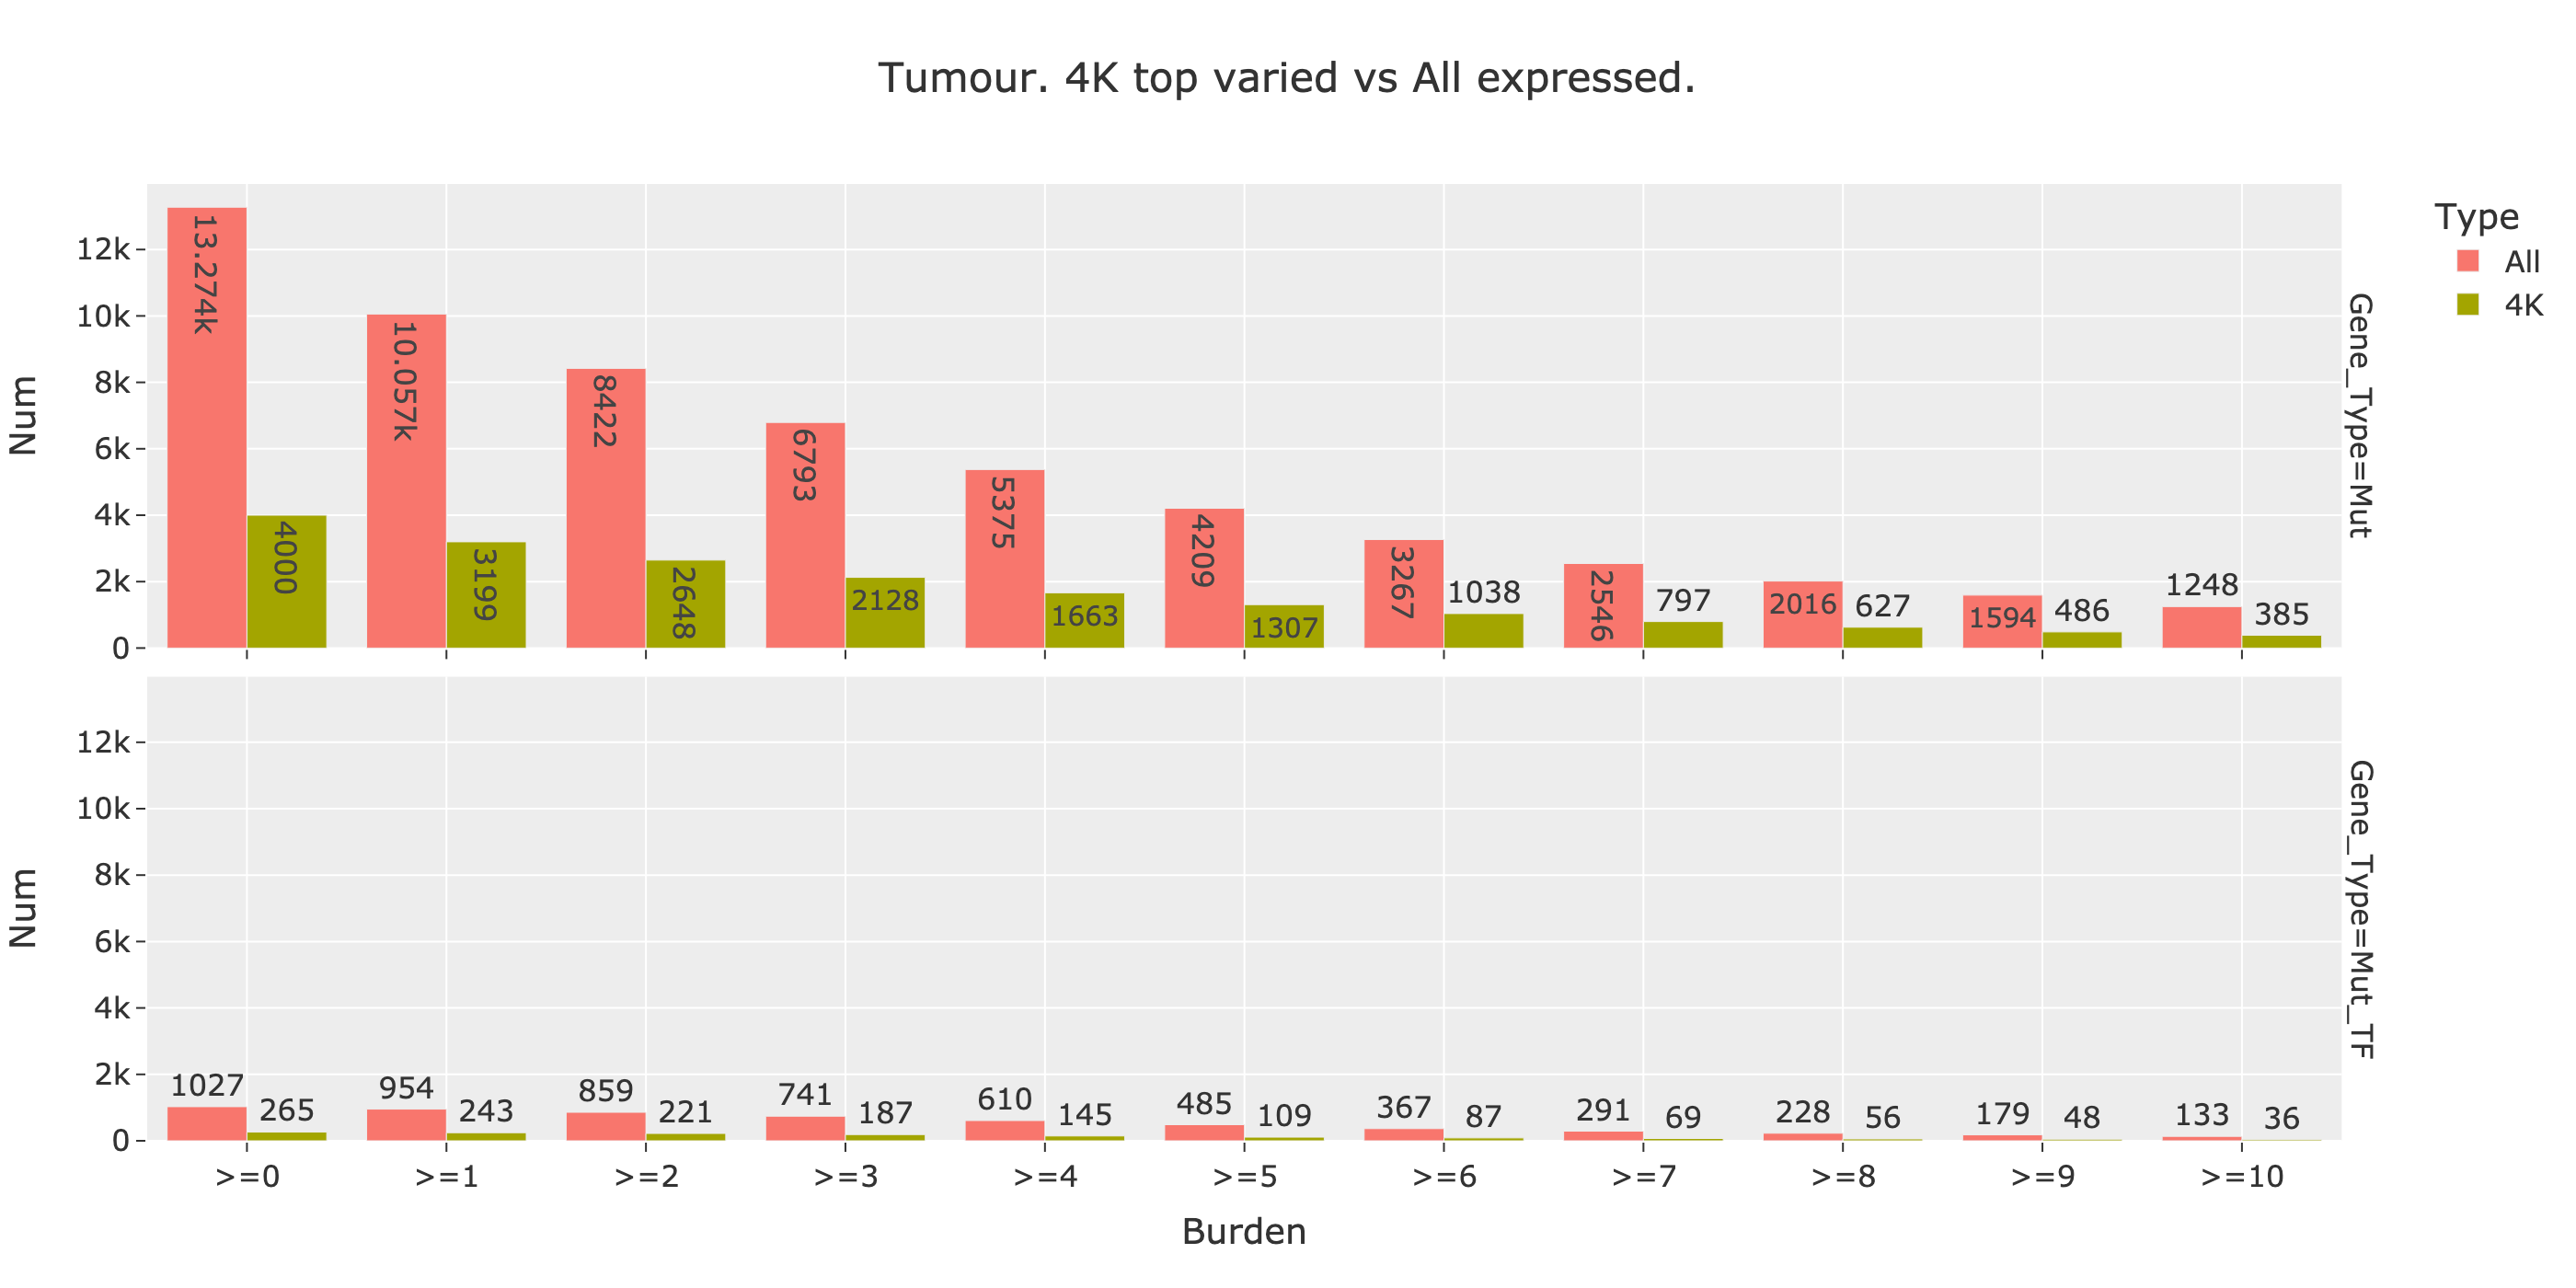
\includegraphics[width=1.0\textwidth,keepaspectratio]{Sections/Network_I/Resources/Tum_network/MutTF_representation_4K-all.png}
    \caption[Mutation representation in most varied genes]{How many genes are mutated in the 4K most varied genes compared to all the expressed genes. First plot includes all the genes expressed in  and non-TF, while the bottom only the TF. Overall the figure shows that there are a few genes with a high mutation burden included in the 4000 genes used to build the networks.}
    \label{fig:N_I:mut_rep_tum}
\end{figure}

% Why are we doing this analysis - understand the mutation burden representation
To further understand how the weight modifiers affect the network, it is essential to check the presence of the mutation burden (i.e., the number of samples with the mutated gene) across the genes in the network. There are $\approx30K$ genes in the MIBC cohort from TCGA from which less than half ($\approx13K$) are considered expressed by the aggressive filtering\footnote{Aggressive filtering refers to the method described in \cref{s:cs:methods} where more than 4 samples have TPM values larger than $0.5$}, of which only 4K-5K genes are used to build a network. It is worth noting that the mutated genes in TCGA contain only non-synonymous changes (Frameshift, Missense and Nonsense), meaning that they are more likely to affect protein function.

% Commenting on the trends
From the $\approx13K$ genes, there are $\approx$10K genes which are mutated at least once, but as the mutation count is increased, there are fewer genes represented as seen in \cref{fig:N_I:mut_rep_tum}. The same trend can be noticed for TF genes, initially 1027 genes in all the expressed genes, from which about a quarter (265) are mutated; the bottom bar plot in \cref{fig:N_I:mut_rep_tum}.

% Implications
TFs are more commonly mutated than other genes, which supports the importance of their dysregulation in bladder cancer. This is depicted by the inverse relationship of the number of TF genes with the mutation burden, e.g., for mutation burden $>=$10, there are 385 of the 4000 genes initially used for building the network ($\sim$10\%) and 36 out of the 265 TF ($\sim$14\%). The trend can be noticed in both all the 4000 genes and the TF, but the latter has a higher representation of the mutated genes, see \cref{fig:N_I:mut_rep_tum}. 

% Linking it back to the weight modifiers
With a low representation of the mutated genes, the weight modifiers might have a limited impact on the network and the MIBC stratification. This is not so explicit in the tumour networks, but it is present in the tumour-derived graphs.


% Leiden stratification
\subsection{Leiden and MIBC stratification} \label{s:N_I:tum_stratification}

% Introducing the algorithm and why I am doing this
% Justify the use of K-means with K = 6
The Leiden algorithm, with Modularity Maximisation, set as the quality function, was applied ten times to study the variability of the community detection algorithm. The three graphs, standard, reward and penalised, were built from the 4,000 most varied genes, with a minimum degree of 3 for standard genes and 6 for TF\footnote{See \cref{s:N_I:sel_tfs} for the experiments and data that support the configuration of 6 edges per TF.}. After applying ModCon to the important genes from the network, K-means clustering (K=6) was performed on the MEV values to identify MIBC subtypes. The group size of 6 was chosen to maintain consistency with previous findings (i.e., the cluster analysis from \cref{s:clustering_analysis}), where six subtypes of MIBC were identified, and to avoid introducing additional variables into the comparisons. This ensures that the methods developed in this chapter are verified against known basal/luminal splits; in the subsequent sections, a cluster analysis is performed \cref{s:p0}. 

This section's set of experiments aimed to understand the changes in the MIBC subtypes resulting from the reward and penalised networks.

% Talk about the number of communities
\paragraph*{Effects to Leiden method}


\begin{figure}[!t]    
    \centering
    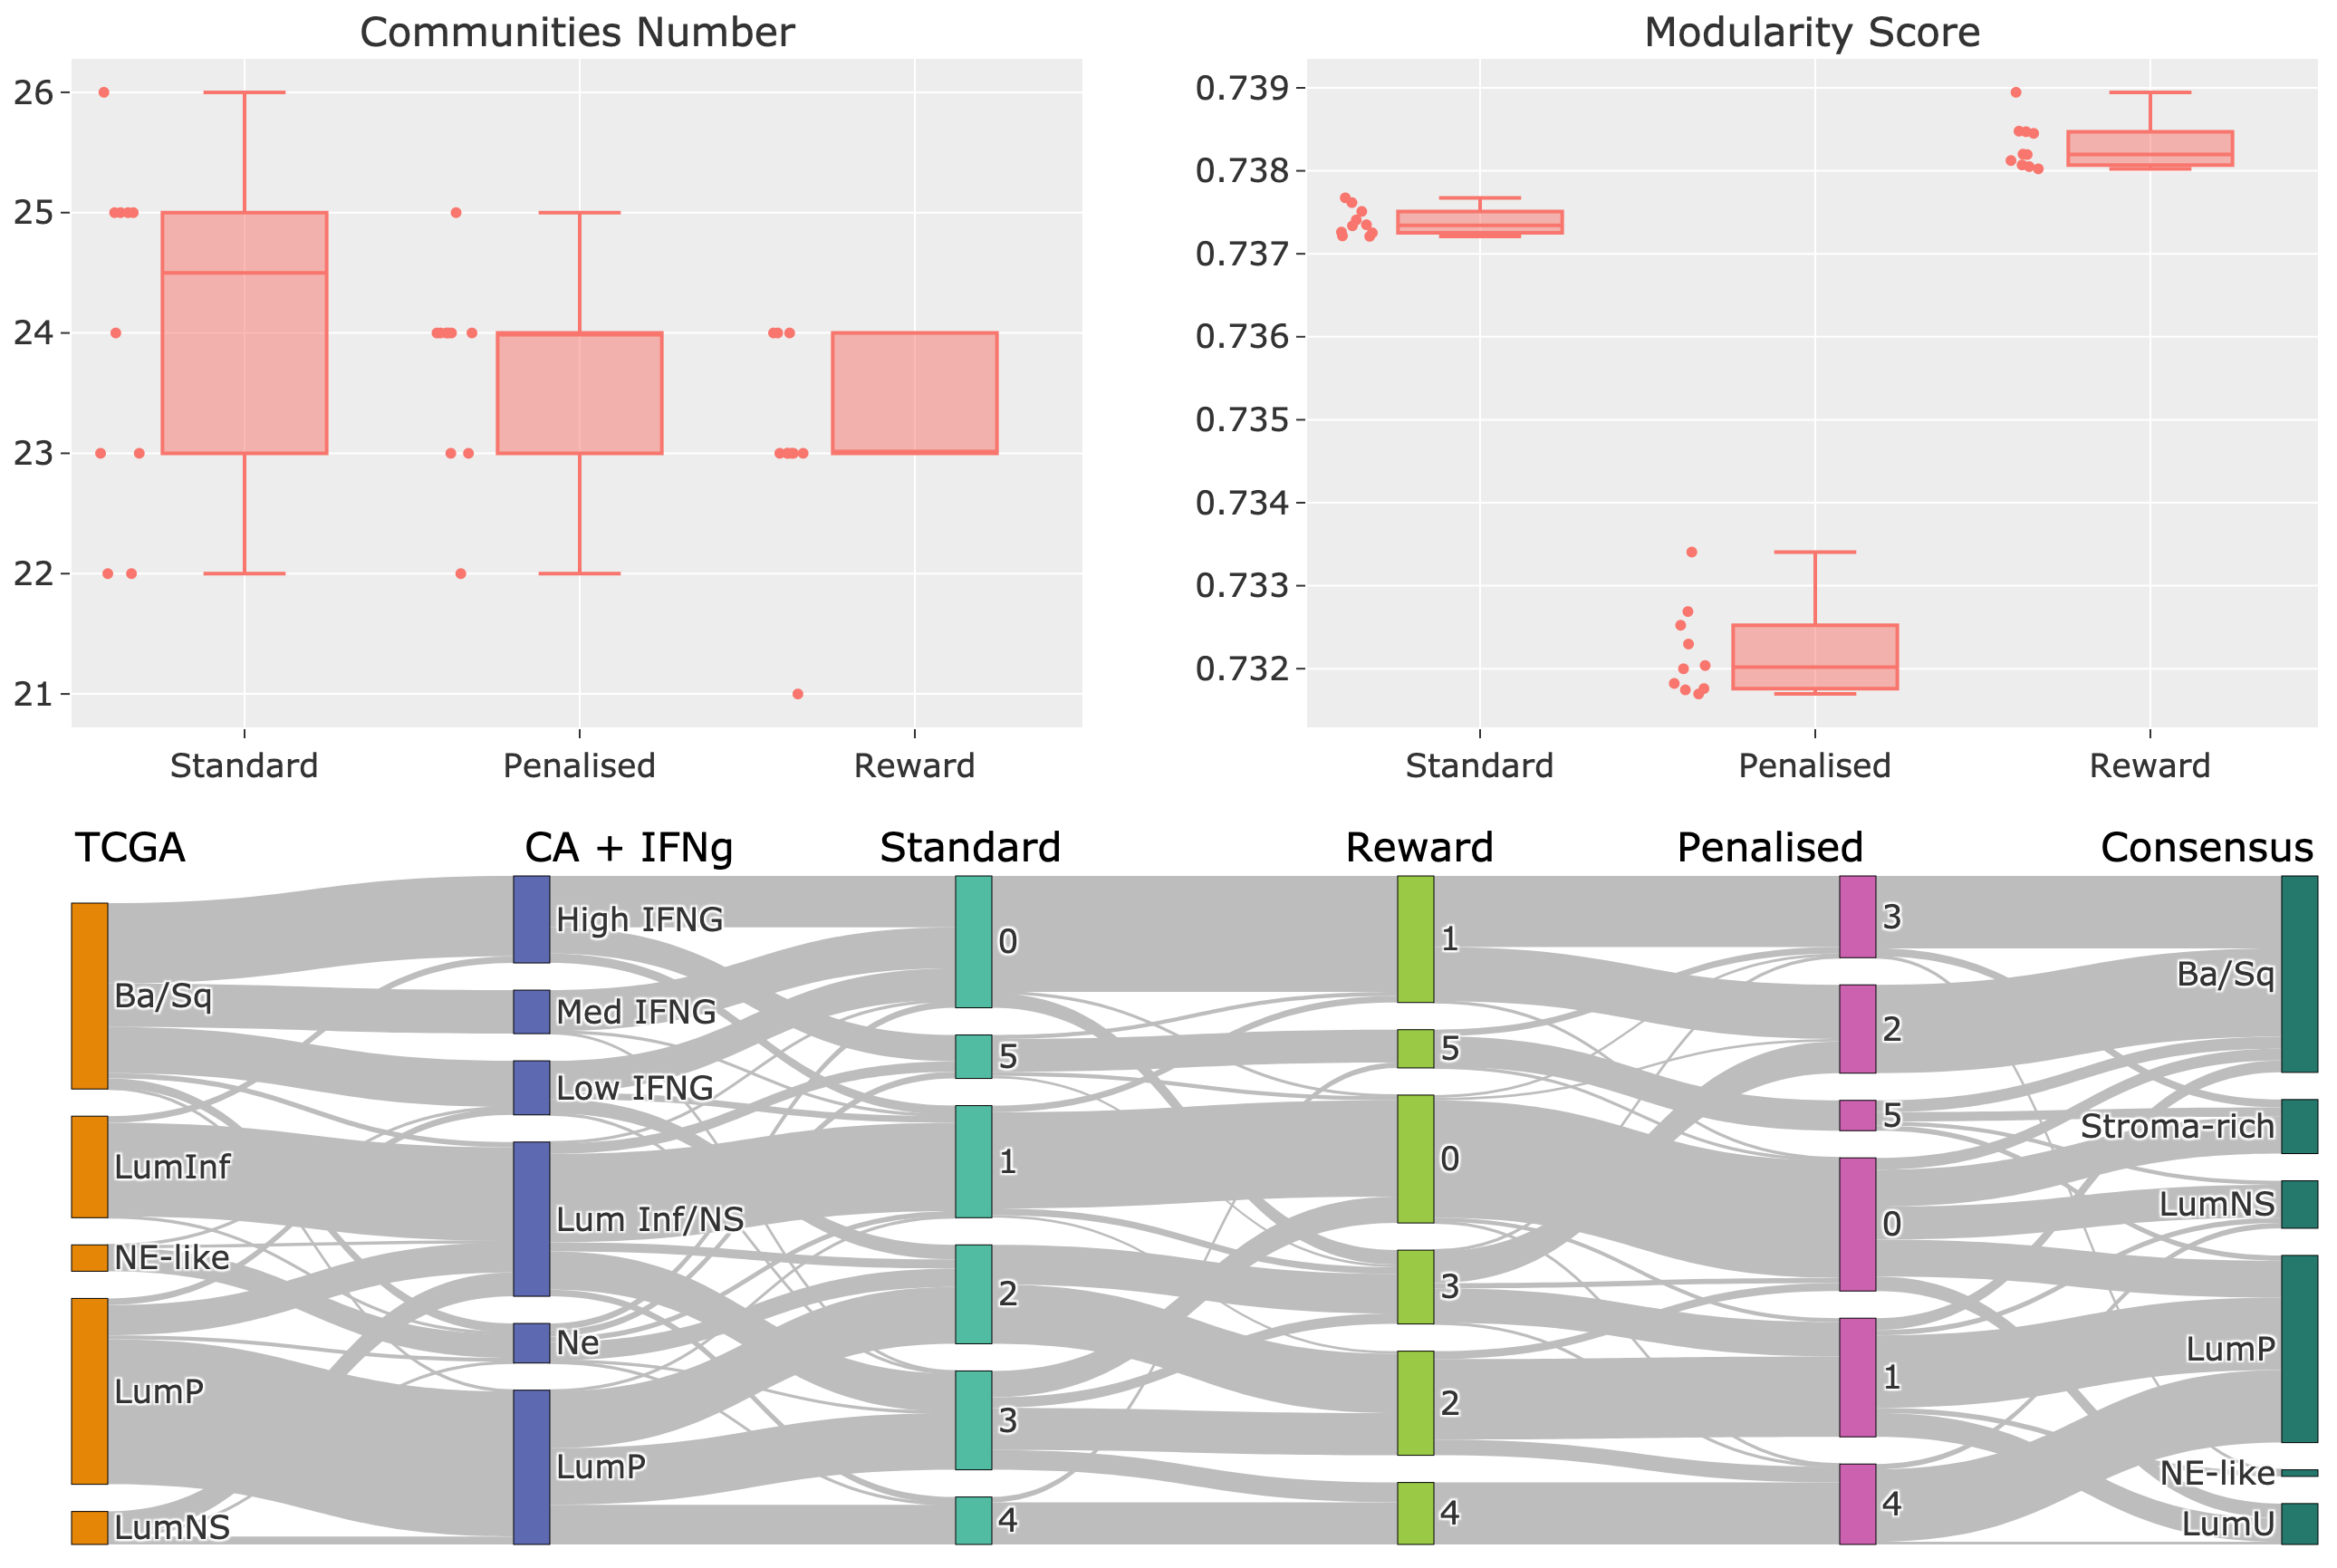
\includegraphics[width=1.0\textwidth,keepaspectratio]{Sections/Network_I/Resources/Tum_network/LeidenMetrics_Sankey_TF-6.png}
    \caption[Tum: Leiden metrics]{On the top are displayed the community size and Modularity Score. The two metrics used to asses effects of the weight modifiers (standard, reward and penalise) to the Leiden algorithm which was applied 10 times to each network type. At the bottom the Sankey plot displays comparison between the MIBC subtyping derived from the different standard classifiers TCG and consensus \citep{Robertson2017-mg,Kamoun2020-tj}, the previous developed subgroups with the cluster analysis \cref{s:clustering_analysis} and the three different networks. The figure shows that the weight modifiers affect the communities found through Leiden and exhibit different subtypes compared to previous classifications.}
    \label{fig:N_I:tum_leiden_modifiers}
\end{figure}


% Modularity Maximisation
The Modularity Maximisation score measures the quality of community separation, thus evaluating the performance of the Leiden community detection algorithm; see \cref{s:lit:comm_detect} for a more detailed overview. The standard and reward networks have higher Modularity scores compared to the penalised network, suggesting that the communities found in these graphs are better-separated results supported by \acrlong{mw} test, which exhibited significant difference, see \cref{tab:N_I:modularity_module_number}. The standard network has the lowest variance in modularity scores, contrasting the stability of Leiden with that of the reward network. The penalised network performs the worst according to the Modularity Maximisation score, consistent with the results from the network metrics explored in the previous section, see \cref{s:N_I:tum_describe}.

There is a non-significant difference (\acrshort{kw}:  3.3047, p-value 0.1915) in the number of communities found by the three networks; for pair-wise MW comparison see \cref{tab:N_I:modularity_module_number}. The Leiden algorithm appears to be more stable in the reward network, while it finds more communities in the standard network when comparing the median values; see \cref{fig:N_I:tum_leiden_modifiers}.


\begin{table}[!t]
  \centering
  \small
  \begin{tabularx}{\textwidth}{>{\hsize=.5\hsize}X|>{\hsize=.5\hsize}X|>{\hsize=.5\hsize}X}
    \toprule
    \textbf{Comparison} & \textbf{Modularity Score} & \textbf{Module Number} \\
    \midrule
    \textbf{Standard vs Reward} & 0.0; $1.83e^{-4}$ & 68.5; 0.156 \\
    \midrule
    \textbf{Standard vs Penalised} & 100.0; $1.83e^{-4}$ & 59.0; 0.506 \\
    \midrule
    \textbf{Reward vs Penalised} & 0.0; $1.83e^{-4}$ & 70.0; 0.109 \\
    \bottomrule
  \end{tabularx}
  \caption[Tum: Leiden network comparisons statistics]{Comparison of Modularity Score and Module Number across Standard, Reward, and Penalised networks. \acrlong{mw} performed between the compared networks gives the first value while the second is the p-value in the cell. The standard and reward networks are significantly better than the penalised networks.}
  \label{tab:N_I:modularity_module_number}
\end{table}


% Introduce the Sankey plot
Overall, the two top box plots shows that the weight modifiers have an effect on the community detection algorithms and on the MIBC stratification are shown on the bottom Sankey plot; \cref{fig:N_I:tum_leiden_modifiers}. It is worth mentioning that the top performing network by Modularity Maximisation is selected for each of the network types and are then compared with classification in the literature TCGA and consensus \citep{Robertson2017-mg,Kamoun2020-tj}, and the previous classification using the cluster analysis in \cref{s:cs:right_config}. 


% Comment on the Sankey
% - Different subtypes but keeping the two main signal: Basal/Luminal across the classification
% - Have some Basal groups
\paragraph*{Effects on MIBC stratification}


All three networks find different clusters compared to the previous classifications, including our own, which immediately suggests that the network pipeline has the potential to identify new groups. Although the two main 'signals' of Basal and Luminal subtypes are preserved across the clusters identified through the network pipeline, it is important to note that the Luminal groups are split into smaller subgroups compared to the cluster analysis from \cref{s:clustering_analysis}. 

% Commenting on the basal
The basal subtypes with different immune response (Low/Med/High IFNG) are not as clearly defined as in the previous cluster analysis, there is still some separation among these samples. Group 5 which predominately contains High IFNG and Luminal Infiltrated samples, is commonly found across all three networks, suggests that it contains the sample with a high infiltration of either immune or stroma cells as many samples were previously classified stroma-rich (TCGA and Consensus). While the High/Med and Low IFNG samples are clustered together in the standard and reward networks, the samples previously classified as Low IFNG are combined with neuroendocrine samples in the reward network and with Luminal samples in the standard and penalised networks. This suggests that the reward network might better isolate the more undifferentiated samples\footnote{See the biological interpretation of the Basal groups from \cref{s:cs:basal_interp}}.

% Linking the difference shown by the weight modifiers
Concurrently, there is difference in the MIBC subgroups found by the three network types suggesting that the weight modifier have an impact to the tumour's stratification. In addition, the two weight modifier strategies exhibit different MIBC groups with the reward network being closer to the standard graph while the penalised network being the most different from the other two. This can be seen best in the split of the Ba/Sq group (consensus) by the penalised network, while the standard \& reward do not discriminate between the two groups. As mentioned earlier all three networks find a small group of Stroma/Basal (5).

Overall, the stratification shown in \cref{fig:N_I:tum_leiden_modifiers} shows the potential of the Network approach of finding different groups from previous stratification work, including the cluster analysis from the previous section \cref{s:clustering_analysis}. The figure also indicates that the weight modifier have an effect on both the Leiden algorithm and the MIBC stratification, where the groups derived with reward closer to the ones from standard, and penalised exhibited larger differences. The graphs do not find the three different immune Basal groups discovered previously but there is a consistent small group, 5, which might be related with cell infiltration, thus showing the potential of the network approach to find new biological relevant groups.


% Nonetheless, there is little difference between the networks suggesting that the weight modifiers do not have a high impact on MIBC stratification with K-means (K=6).

% Further commenting on the Sankey
% As it was mentioned earlier that the two main Basal and Luminal 'signals' are found in the the subtypes derived from the three networks. The \acrfull{lump} is split into two smaller groups across with varying sizes, while the Luminal Infiltrated (from the previous clustering analysis) is also consistently found by the three networks.

% There are more changes in the Basal (TCGA/consensus) and \acrfull{ne}. The Standard and Reward are consistent in finding the same 3 groups (\textbf{0, 3, 5}) where \textbf{1/0} is a mixed of LumInf/NS and High IFNg, \textbf{4} is mainly Low IFNG and a few NE samples while \textbf{2} is a combination of High and Medium IFNg. This may suggest that cluster 4 represents the tumours which are more basal (de-differentiated), while \textbf{5} the tumours with high infiltration and immune response and cluster \textbf{2} the samples between the two. In the Penalised network sub-grouping the cluster \textbf{5} remains the same, but \textbf{4} and \textbf{1} are changed. The former contains more of the LumP and Low IFNG samples, while the latter hold most of the IFNG samples. This suggest that the Penalised network stratification perform worst.


% cluster analysis vs network gene selection
\subsection{Cluster analysis vs network gene selection} \label{s:N_I:cs_vs_gene_sel}

% Network as a gene selction
The network pipeline developed in this section can be thought as a sophisticated gene selection mechanism based on multiple data-types: gene co-expression, mutation and transcription factors. Specifically as the ModCon step from  \cref{fig:N_I:network_pipeline} picks the genes that have the highest connectivity (see \cref{eq:modcon}), which are then used for cluster analysis (through MEV). Similarly, in the previous chapter $\approx$3K top most relative varied genes were used in the K-means cluster analysis. Therefore, there is a need to compare the two gene selection methods and to assess the differences.

% What's the comparison
The comparison is performed only using TCGA's MIBC dataset to avoid gene expression differences introduced by the healthy samples. The network was constructed from the 5K most varied genes, no weight modifier and the minimum degree for TF  was set to 6\footnote{The Selective Edge pruning experiments from \cref{s:N_I:sel_pruning} showed diminished returns from allowing more than 6 edges per TF.} and 3 to the standard genes. For a network formed of 5K genes, the ModCon (=100 for each community) selects in total $\approx$2.8K genes which is comparable with the 3K most relative varied genes. Note, in the cluster analysis work from \cref{s:clustering_analysis} 3500 genes were used. Thus, the network size was increased and the number of genes selected was reduced so that the gene sets are comparable.

\begin{figure}[!t]    
    \centering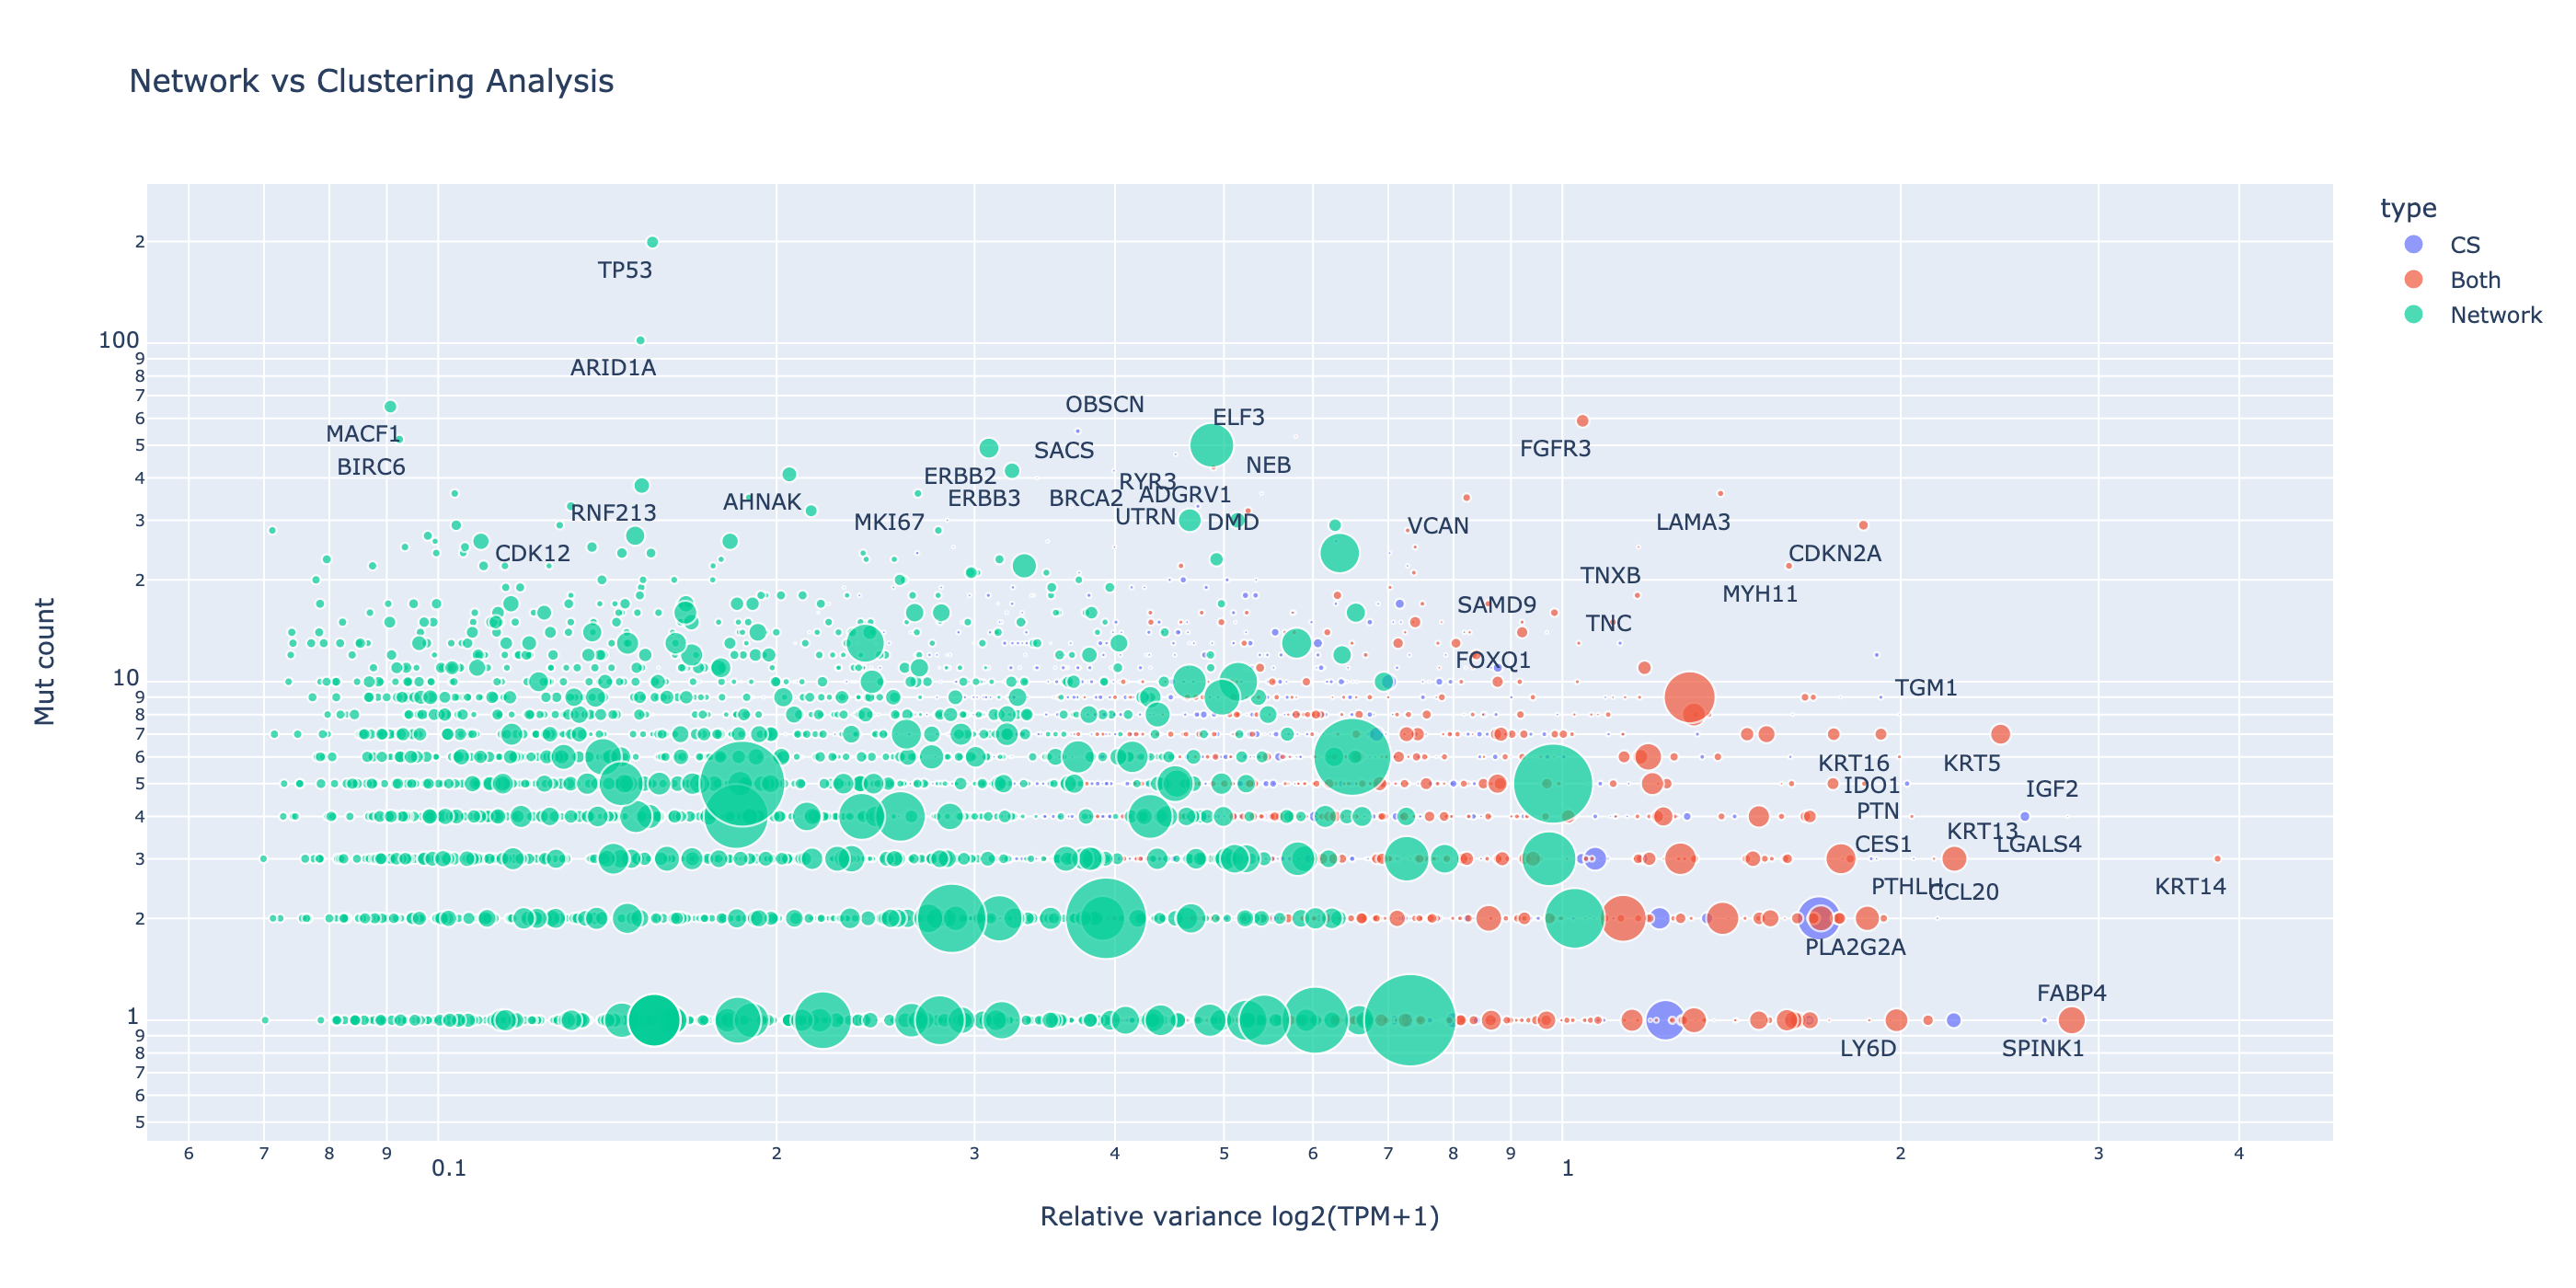
\includegraphics[width=1.0\textwidth,keepaspectratio]{Sections/Network_I/Resources/Tum_network/ClusteringAnalysis_vs_Network_3.png}
    \caption[Gene selection: network vs cluster analysis]{Network selection vs. Cluster Analysis. Red points are represented by the genes selected exclusively by the highest median standard deviation ratio, the green by the network and mustard by both approaches. The size of the points is the median expression of the genes across TCGA sample. To avoid log values of 0 the mutations count were offset by one. Showing that the network approach selects genes that are not only highly varied but also have higher median expression and mutation burden.}
    \label{fig:N_I:network_ca_selection}
\end{figure}

% Interpret the results
There are 2053 different genes and 747 shared between the two sets of genes, which are all shown in the variance vs. mutation burden scatter plot from \cref{fig:N_I:network_ca_selection}. As expected, the genes selected only by relative variance are skewed to the right picking of highly mutated genes with a high variance. By contrast, the network approach selects most of the varied genes and some of the highest mutated genes despite having low variance. The points' size is relative to the median expression in TCGA cohort, and from \cref{fig:N_I:network_ca_selection}, it can be seen that the canonical gene selection does not include the highly expressed genes as the network does.

The large difference between the genes selected is explained by that the network approach does not select only highly varied genes but also the ones that have consistent expression values and high mutation burden. This means that the network method introduced in this chapter can select genes with more diverse molecular properties than the other methods, which may lead to newer and different MIBC subgroups.


\subsection{Summary}

% Effect on the network metrics and communities
The two sets of experiments performed in this section suggest the potential of a network-based approach to stratify MIBC. The three different networks—standard, reward, and penalised—were validated using various network and community detection metrics \cref{fig:N_I:net_metrics_tum,fig:N_I:tum_leiden_modifiers}. Both analyses demonstrated that the weight modifiers affect both the nodes' properties (e.g., degree, closeness) and the Leiden algorithm.

% MIBC subtyping
The MIBC subgroups derived from the three networks differed from existing classifications, highlighting the potential to identify new subtypes. Compared to the previous cluster analysis in \cref{s:clustering_analysis}, the networks were unable to identify the three Basal immune groups but showed promise for uncovering new biology, as evidenced by the identification of a small group, 5, which contained samples previously classified as Stroma. Additionally, the two different edge weight modifiers revealed distinct groups from each other and the standard network, indicating the effect of mutations in the network.

% Gene selection
Following this, the differences in gene selection between the cluster analysis and the network approach were explored, as depicted in \cref{fig:N_I:network_ca_selection}. This comparison shows that the network is capable of selecting genes with a wider range of properties. Genes with higher mutation burdens, greater magnitudes, and higher variance are selected by the network approach, while the standard approach tends to select only those with the highest relative variance.

Overall, the experiments in this section demonstrated the advantages of the network approach as a method for cancer subtyping and the effects of integrating mutation data by modelling edge weights. The following section will explore the data integration at network level.
